 \documentclass[letterpaper]{tufte-book}
\usepackage{booktabs}
\usepackage{tabularx}
\usepackage{longtable} 
\usepackage{lscape}
\usepackage{colortbl}
\usepackage{graphicx}
\graphicspath{ {../images/} }

\geometry{
  left=.5in,
  right=.5in,
  top=.5in,
  bottom=.5in
}

%\title{Identifying Causal Scenarios}

\begin{document}

\begin{landscape}
\advance\vsize0cm
\csname @colroom\endcsname=\vsize
\textheight=\vsize
\csname @colht\endcsname=\vsize

\setlength{\parindent}{0em}
\setlength{\parskip}{.75em}

\begin{multicols}{2}
[ \section{Identifying Causal Scenarios}]

\newthought{Definition}

Now we ask, ?What could cause an operator or part of the system to take an inappropriate action or fail to take action when needed?? A \textbf{causal scenario} is a description of how and why the \textbf{unsafe control action} could happen.

For each \textbf{unsafe control action}, we will inspect the \textbf{control loop} that action is part of in the \textbf{hierarchical control model}, indentifying how flaws in that control loop could cause that action to occur in that particular inappropriate way.

Consider each of the control loop flaws, or \textbf{causal factors}, marked on the control loop diagram, and ask ?How could that factor contribute to this unsafe control action?? 

Once we have a list of causal scenarios, we can check whether our system has mechanisms to address them.

\newthought{Causal Factors Prompt}

[Based on a diagram from\emph{Engineering A Safer World} p.223]
\begin{center}
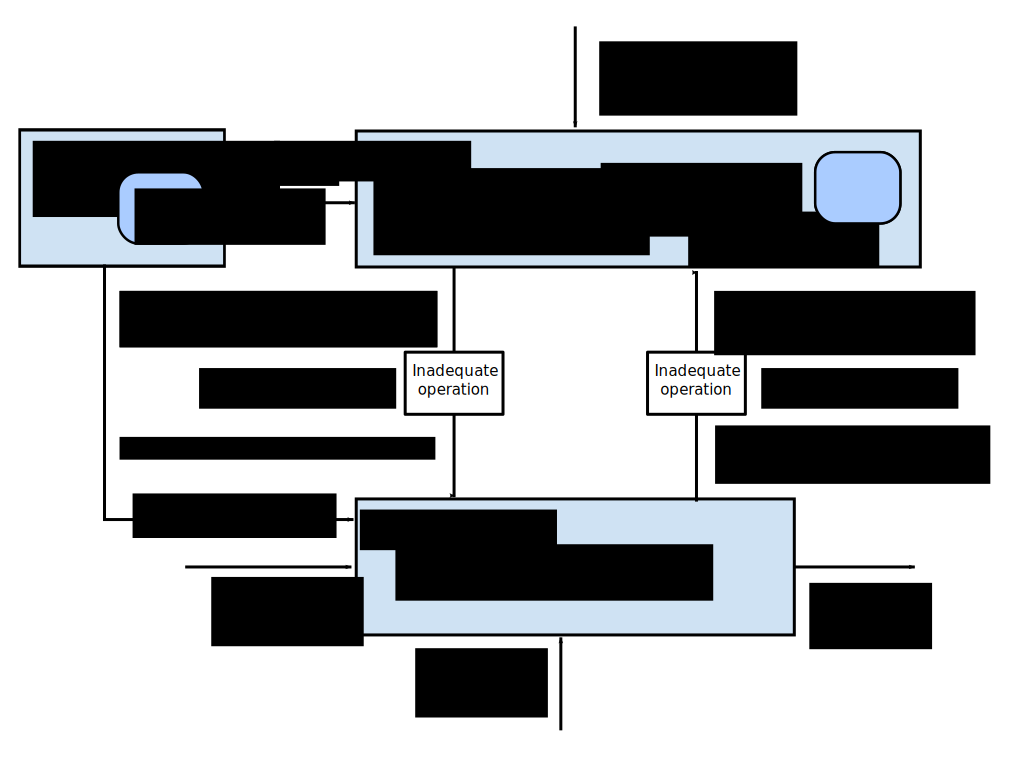
\includegraphics[width=9cm]{generic_control_loop-flaws}
\end{center}

\columnbreak

\newthought{Desired Qualities}

\begin{compactitem}
\item Completeness --- When finding causal scenarios for a particular unsafe control action, consider each part of the control loop in which the action occurs.
\item Plausibility --- Could this happen at all?
\item Relevance
\end{compactitem}

\newthought{Strategic Approaches} 

This is an exercise in focused brainstorming; we might not think of everything, but focusing on the system bit by bit may make it easier to come up with potential problems we hadn?t considered earlier.

\begin{compactitem}
\item \textsc{Divide and conquer} --- This work can be split up among several people.
\item \textsc{Pace your efforts} --- Track progress, returning later as needed.
\item \textsc{Triage and prioritize} --- Prioritize investigating actions needing additional scrutiny, e.g. actions that are new, poorly understood, currently changing, be-lieved to be risky, or involved in close interactions with other systems that need additional scrutiny.
\end{compactitem}  

\emph{Toolkit}: Causal Factors diagram

\newthought{Relationship to other concepts}

Each \textbf{unsafe control action} maps to several \textbf{causal scenarios}.

Each \textbf{causal scenario} maps to at least one unsafe control action.

When performing this step, we use the \textbf{hierarchical control model} to identify system parts relevant to the action being inspected.

When we check our list of causal scenarios to see whether our system has mechanisms to address them, we identify new system requirements.

\pagebreak

 \newthought{Thermostat Example}
 

\textbf{Unsafe Control Action}: Turning the heat ON when the room is already too hot.

\textbf{Causal Scenarios}:

\begin{compactitem}
\item Control input or external info is wrong or missing:
  
  TARGET temperature is not set by the user and the default is unusually high.
  TARGET temperature is set to the wrong value; the user believed the input was in Farenheit, but the thermostat was using Celsius.  

\item Controller: Inadequate Control Algorithm.
  
Too long a delay between when thermostat measures temperatures and when it acts, so that the room has heated up (e.g. due to warm sunlight) before the thermostat turns the heater on.  
\item Controller: Process Model Inconsistent, incomplete, or incorrect.

  Perhaps the controller is storing temperature in Celsius, while the TARGET temperature is in Farenheit.
  Perhaps only two digits of temperature are stored and the room is 103F.
\item Inadequate or missing feedback:

  Thermometer uses different units than the thermostat, reporting degrees C which are recorded as degrees F.
  Thermometer is disconnected and the thermostat has not updated its MEASURED temperature.
%\item Feedback Delays
%
%MEASURED temperature is consistently delayed. MEASURED(t) temperature is ACTUAL(t-Delta). MEASURED temperature is inconsistently delayed.
 \item Sensor: inadequate operation; incorrect or no information provided

   Perhaps the thermometer is in an unusually cold location, unrepresentative of the general room temperature, so the thermostat activates the heat even when the room at large is already warm.
\end{compactitem}

\columnbreak
Other examples, not necessarily relevant to this action:

\begin{compactitem}
\item Controlled Process: Component failures
   
Furnace is broken. Furnace is out of fuel.
   \item Unidentified or out-of-range disturbance
   
Water in the basement, missing roof or walls, open windows
\item Actuator: Inadequate operation

  Heater failed to turn HEAT ON when signaled. Baseboards not radiating heat. Leaking water. Frozen pipes.

\item Controller 2: Conflicting control actions

Perhaps someone manually turned the heater on, circumventing the thermostat.
\end{compactitem}

 
\end{multicols}
\end{landscape}
\end{document}
